\documentclass[a4paper,12pt]{article}
\usepackage[english]{babel}
\usepackage{graphicx}
\usepackage{tikz}
\usepackage{wrapfig}
\usepackage{array}
\usepackage{color} 
\usepackage{hyperref}
\usepackage{enumitem}
\usepackage[normalem]{ulem}
\usepackage[font=small,labelfont=bf]{caption}
\usepackage{tcolorbox}
\hypersetup{
    colorlinks,
    citecolor=black,
    filecolor=black,
    linkcolor=black,
    urlcolor=blue
}
\usepackage{changepage}
\addto{\captionsenglish}{\renewcommand{\refname}{}}

\begin{document}

\title{%
  Group Project Part 3 - ElasticSearch \\
  \large of Systems and Methods for Big
    and Unstructured Data Course \\(SMBUD)\\
    held by\\ Brambilla Marco\\ Tocchetti Andrea \\
  \vspace{5mm}
  \Large \textbf{Group 14}}
\author{Banfi Federico\\
  \texttt{10581441}
  \and
  Carotenuto Alessandro\\
  \texttt{10803080}
  \and
  Donati Riccardo\\
  \texttt{10669618}
  \and
  Mornatta Davide\\
  \texttt{10657647}
  \and
  Zancani Lea\\
  \texttt{10608972}}
\date{Academic year 2021/2022}
\maketitle
\begin{center}
  \includegraphics[width=4cm]{polilogo.png}\\
\end{center}
\newpage
\tableofcontents
\newpage
\section{Problem Specification}
\paragraph{}The use of Big Data is not limited exclusively to the tracking and profiling of vast amounts of data to obtain information useful for practical purposes - as seen in previous deliveries - but are also fundamental in the field of research and of statistical studies. This time, in fact, our project is focused on the use of an Information Retrieval system specifically designed to the collection and the in-depth study of data to obtain more precise and meaningful analyzes. \par
In particular, the ElasticSearch search engine will be used to monitor the spread of the SARS-CoV-2 virus in recent times from a global point of view and to track the progress of the vaccination campaign from a perspective no longer linked to individuals but to a larger scale. Thanks to the IR-based approach on which it is based, ElasticSearch is the most suitable system for this kind of task as, compared to other SQL and NoSQL solutions, it gives the possibility to compute more accurate searches by exploiting the main features available: the full-text search and the ranking strategy used to evaluate the relevance of the results obtained, which guarantee more wide-ranging query outcomes in order of "importance".
\section{Hypotheses}
\paragraph{} This time, pre-existing datasets released by various government authorities with large amounts of data collected over the last few years were examined, moreover, in order to obtain significant results and realistic information in executing the queries, a time interval was taken at least 3 months. The datasets considered are:
  \begin{enumerate}[noitemsep]
    \item \href{https://raw.githubusercontent.com/italia/covid19-opendata-vaccini/master/dati/somministrazioni-vaccini-latest.csv}{administration-vaccines-latest.csv} issued by the \emph{"Commissione Straordinaria per la gestione l’emergenza Covid-19"} appointed by the Italian Government,
    \item \href{https://raw.githubusercontent.com/pcm-dpc/COVID-19/master/dati-regioni/dpc-covid19-ita-regioni.csv}{dpc-covid19-ita-regions.csv} issued by the \emph{"Dipartimento della Protezione Civile"} in accordance with the rules established by the \emph{"Presidenza del Consiglio dei Ministri"} and the \emph{"Ministero della Salute della Repubblica Italiana"} regarding the Covid-19 emergency,
    \item \href{https://www.ecdc.europa.eu/en/publications-data/data-virus-variants-covid-19-eueea}{SARS-CoV-2-variants-data-in-EU-EEA.csv} issued by the \emph{"European Center for Disease Prevention and Control"},
    \item \href{https://raw.githubusercontent.com/owid/covid-19-data/master/public/data/owid-covid-data.csv}{owid-covid-data.csv} released by the Oxford University research group that manages the scientific online publication website \emph{ourworldindata.org}, the data collected comes from various institutions such as the \emph{"Center for Systems Science and Engineering (CSSE) at Johns Hopkins University"}.
   \end{enumerate}
\newpage
\paragraph{} The datasets are in .csv format and can be found in the WRITE FOLDER folder, two of these contain data relating to the administration of vaccines and cases ascertained for the Italian national territory only, while the other two relate to the spread of SARS-CoV-2 variants in Europe and the global pandemic trend around the world.
\section{Dataset Schemata}
\paragraph{} During the import of the data present within each dataset, it was preferred to take advantage of the Automatic Mapping feature available on ElasticSearch, subsequently checking that there were no compatibility problems with the types of the various fields. Furthermore, for those fields that expected String data, the keyword type was used instead of full-text to obtain more precise and targeted results by executing the queries. Below are the tables with the diagrams of the various datasets produced following the Mapping, some fields have been omitted for the sake of brevity (to test the queries not all fields have been taken into consideration and reporting them all in the following tables would have been superfluous), however, it is possible to view the complete diagrams of each dataset with all the fields in the FOLDER NAME folder.
\subsection{administration-vaccines-latest.csv}
\paragraph{}
\begin{center}
\begin{tabular}{|m{45mm}|>{\raggedright}m{16mm}|m{75mm}|}
\hline
\multicolumn{1}{|c|}{\textbf{ Field Name }}
& \multicolumn{1}{c|}{\textbf{ Data Type }} 
    	& \multicolumn{1}{c|}{\textbf{ Description }}\\
\hline
fornitore & String & Complete name of the supplier of the vaccine \\
\hline
data\_somministrazione & Datetime & Administration date of the vaccines \\
\hline
fascia\_anagrafica & String & Age group of the people administered with the vaccines \\
\hline
sesso\_maschile & Long & Number of vaccinations administered to males \\
\hline
sesso\_femminile & Long & Number of vaccinations administered to females \\
\hline
\end{tabular}
\end{center}

\begin{center}
\begin{tabular}{|m{45mm}|>{\raggedright}m{16mm}|m{75mm}|}
\hline
prima\_dose & Long & Number of people administered with the first dose \\
\hline
seconda\_dose & Long & Number of people administered with the second dose \\
\hline
pregressa\_infezione & Long & Number of people administered with a dose after they have
been infected \\
\hline
dose\_addizionale\_booster & Long & Number of people administered with an additional dose/recall \\
\hline
codice\_NUTS1 & String & Nomenclature of Territorial Units for Statistics code (Groups of regions) \\
\hline
nome\_area & String & Name of the region \\
\hline
\end{tabular}
\end{center}

\subsection{dpc-covid19-ita-regions.csv}
\paragraph{}
\begin{center}
\begin{tabular}{|m{45mm}|>{\raggedright}m{16mm}|m{75mm}|}
\hline
\multicolumn{1}{|c|}{\textbf{ Field Name }}
& \multicolumn{1}{c|}{\textbf{ Data Type }} 
    	& \multicolumn{1}{c|}{\textbf{ Description }}\\
\hline
data & Datetime & Date of observation \\
\hline
denominazione\_regione & String & Name of the Region \\
\hline
terapia\_intensiva & Long & Intensive Care \\
\hline
totale\_ospedalizzati & Long & Total hospitalised patients \\
\hline
totale\_positivi & Long & Total amount of current positive cases \\
\hline
variazione\_totale\_positivi & Long & News amount of current positive cases \\
\hline
nuovi\_positivi & Long & News amount of current positive cases \\
\hline
deceduti & Long & Death \\
\hline
\end{tabular}
\end{center}

\newpage
\subsection{SARS-CoV-2-variants-data-in-EU-EEA.csv}
\paragraph{}
\begin{center}
\begin{tabular}{|m{45mm}|>{\raggedright}m{16mm}|m{75mm}|}
\hline
\multicolumn{1}{|c|}{\textbf{ Field Name }}
& \multicolumn{1}{c|}{\textbf{ Data Type }} 
    	& \multicolumn{1}{c|}{\textbf{ Description }}\\
\hline
new\_cases & Long & Weekly number of new confirmed cases \\
\hline
number\_detections\_variant & Long & Number of detections reported of the variant \\
\hline
number\_sequenced & Long & Weekly number of sequences carried out \\
\hline
number\_sequenced \_known\_variant & Long & Weekly number of known variant sequences carried out \\
\hline
source & String & Data source, either GISAID EpiCoV database or TESSy \\
\hline
variant & String & Each VOC (\emph{"variants of concern"}, i.e. those considered the most lethal), Other or UNK \\
\hline
year\_week & String & Year and week of reference \\
\hline
\end{tabular}
\end{center}

\subsection{owid-covid-data.csv}
\paragraph{}
\begin{center}
\begin{tabular}{|m{45mm}|>{\raggedright}m{16mm}|m{75mm}|}
\hline
\multicolumn{1}{|c|}{\textbf{ Field Name }}
& \multicolumn{1}{c|}{\textbf{ Data Type }} 
    	& \multicolumn{1}{c|}{\textbf{ Description }}\\
\hline
new\_cases & Long & New confirmed cases of COVID-19 \\
\hline
new\_deaths & Long & New deaths attributed to COVID-19 \\
\hline
location & String & Geographical location \\
\hline
date & Datetime & Date of observation \\
\hline
new\_cases\_per\_million & Long & New confirmed cases of COVID-19 per 1,000,000 people \\
\hline
\end{tabular}
\end{center}
\newpage

\section{Queries and Commands}
\subsection{Queries}
\paragraph{} In all the queries performed in an index with a timestamp we are going to filter the documents only considering the 4 months period that we are analysing. For readability we won't represent this part in the next queries.
\begin{tcolorbox}[colback=pink!5!white,colframe=pink!75!black,title=FILTER]
\begin{verbatim}
  . . .
 "query": {
   "bool": {
     "must": [
       {
         "range": {
           "data_somministrazione": {
             "gte": "2021-08-25T00:00:00Z+01",
             "lte": "2021-12-25T00:00:00Z+01"
           }
         }
       }
     ]
   }
 },
 . . .
\end{verbatim}
\end{tcolorbox}
\newpage

\subsubsection{Total number of vaccinations ordered per day [VACCINES INDEX]}
\paragraph{} This query allows us to retrieve an ordered list containing the total number of vaccinations ( first + second + booster + previous infection ) per day.
\begin{tcolorbox}[colback=green!5!white,colframe=green!75!black,title=QUERY]
\begin{verbatim}
GET /vaccines/_search
{
  "size":0,
 "aggs": {
   "vacc_by_date": {
     "terms": {
       "field": "data_somministrazione",
       "order": {"Totale_dosi": "desc"}
     },
     "aggs" : {
        "Totale_dosi" : { "sum" : { "script" : "
         doc['prima_dose'].value +
         doc['seconda_dose'].value + 
         doc['dose_addizionale_booster'].value +
         doc['pregressa_infezione'].value" } }
     }
   }
 }
}
\end{verbatim}
\end{tcolorbox}
\newpage

\paragraph{} The output is given by: 
\begin{itemize}[noitemsep]
\item[•] The Date as a key
\item[•] The doc count
\item[•] The total number of vaccinations
\end{itemize}
\begin{tcolorbox}[colback=red!5!white,colframe=red!75!black,title=OUTPUT]
\begin{verbatim}
 "aggregations" : {
    "vacc_by_date" : {
      "doc_count_error_upper_bound" : -1,
      "sum_other_doc_count" : 48995,
      "buckets" : [
        {
          "key" : 1639612800000,
          "key_as_string" : "2021-12-16T00:00:00.000Z",
          "doc_count" : 413,
          "Totale_dosi" : {
            "value" : 584181.0
          }
        },
        {
          "key" : 1639699200000,
          "key_as_string" : "2021-12-17T00:00:00.000Z",
          "doc_count" : 417,
          "Totale_dosi" : {
            "value" : 578422.0
          }
        },
        . . .
\end{verbatim}
\end{tcolorbox}
\newpage

\subsubsection{Total number of vaccinations group by region and provider [VACCINES INDEX]}
\paragraph{} This query (performed on the vaccines index) allows us to retrieve the total number of vaccinations, as the previos one, grouped by region and provider of the vaccine.
\begin{tcolorbox}[colback=green!5!white,colframe=green!75!black,title=QUERY]
\begin{verbatim}
GET /vaccines/_search
{
  "size":0,
 "aggs": {
   "vacc_by_date": {
     "terms": {
       "field": "nome_area"
     },
     "aggs": {
       "s": {
         "terms": {
           "field": "fornitore",
            "order": {"Totale_dosi": "desc"}
         },
         "aggs" : {
            "Totale_dosi" : { "sum" : { "script" : "
            doc['prima_dose'].value + 
            doc['seconda_dose'].value + 
            doc['dose_addizionale_booster'].value + 
            doc['pregressa_infezione'].value" } }
        }
       }
     }
   }
 }
}
\end{verbatim}
\end{tcolorbox}
\newpage

\paragraph{} The output is given by: 
\begin{itemize}[noitemsep]
\item[•] The name of the region
\item[•] The names of the providers with the total related vaccinations
\begin{tcolorbox}[colback=red!5!white,colframe=red!75!black,title=OUTPUT]
\begin{verbatim}
"buckets" : [
        {
          "key" : "Lazio",
          "doc_count" : 9852,
          "s" : {
            "doc_count_error_upper_bound" : 0,
            "sum_other_doc_count" : 0,
            "buckets" : [
              {
                "key" : "Pfizer/BioNTech",
                "doc_count" : 3238,
                "Totale_dosi" : {
                  "value" : 7622311.0
                }
              },
              {
                "key" : "Moderna",
                "doc_count" : 2984,
                "Totale_dosi" : {
                  "value" : 1418839.0
                }
              },
              . . .
\end{verbatim}
\end{tcolorbox}
\end{itemize}
\newpage

\subsubsection{Astrazeneca doses grouped by age range [VACCINES INDEX]}
\paragraph{} This query allows us the monitor the vaccinations of the provider Astrazeneca in the different age ranges.
\begin{tcolorbox}[colback=green!5!white,colframe=green!75!black,title=QUERY]
\begin{verbatim}
GET /vaccines/_search
{
  "size":0,
  "aggs": {
    "aggr1": {
      "terms": {
        "field": "fascia_anagrafica"
      },
      "aggs" : {
            "Totale_dosi" : { "sum" : { "script" : "
            doc['prima_dose'].value + 
            doc['seconda_dose'].value + 
            doc['dose_addizionale_booster'].value + 
            doc['pregressa_infezione'].value" } }
        }
    }
  }
}
\end{verbatim}
\end{tcolorbox}
\newpage

\paragraph{} The output is given by: 
\begin{itemize}
\item[•] The age range
\item[•] The total number of Astrazeneca vaccinations
\end{itemize}
\begin{tcolorbox}[colback=red!5!white,colframe=red!75!black,title=OUTPUT]
\begin{verbatim}
"buckets" : [
        {
          "key" : "60-69",
          "doc_count" : 481,
          "Totale_dosi" : {
            "value" : 7382.0
          }
        },
        {
          "key" : "70-79",
          "doc_count" : 417,
          "Totale_dosi" : {
            "value" : 3314.0
          }
        },
        . . .
\end{verbatim}
\end{tcolorbox}
\newpage

\subsubsection{Find all the informations about the vaccinations in Lombardia on the 25-11-2021 [VACCINES INDEX]}
\paragraph{} This query allows us the retrieve some specific information about the vaccinations in a certain region, a certain day.
\begin{tcolorbox}[colback=green!5!white,colframe=green!75!black,title=QUERY]
\begin{verbatim}
GET /vaccines/_search
{
  "query": {
    "bool": {
      "must": [
        {
          "term": {
            "data_somministrazione": {
              "value": "2021-11-25T00:00:00"
            }
          }
        },
        {
          "term": {
            "nome_area": {
              "value": "Lombardia"
            }
          }
        }
      ]
    }
  }
}
\end{verbatim}
\end{tcolorbox}
\newpage

\paragraph{} The output is given by: 
\begin{itemize}[noitemsep]
\item[•] The number of documents that match the query
\item[•] The fields of the documents that match the query
\end{itemize}
\begin{tcolorbox}[colback=red!5!white,colframe=red!75!black,title=OUTPUT]
\begin{verbatim}
  "hits" : {
    "total" : {
      "value" : 20,
      "relation" : "eq"
    },
    "max_score" : 3.8716726,
    "hits" : [
      {
        "_index" : "vaccines",
        "_type" : "_doc",
        "_id" : "mVXh7H0BdN5GzFyWWMIo",
        "_score" : 3.8716726,
        "_source" : {
          "area" : "LOM",
          "codice_regione_ISTAT" : 3,
          "nome_area" : "Lombardia",
          "data_somministrazione" : "2021-11-25",
          . . .
\end{verbatim}
\end{tcolorbox}
\newpage

\subsubsection{Find all the vaccinations not in the islands in the age range 80+ [VACCINES INDEX]}
\paragraph{} This query also allows to perform a search of specific documents in the database. i.e. the vaccinations that didn't take place in the islands (NUTS code != ITG) for the age range of 80+ years. 
\begin{tcolorbox}[colback=green!5!white,colframe=green!75!black,title=QUERY]
\begin{verbatim}
GET /vaccines/_search
{  
   "query": {
     "bool": {
       "filter": [
         {
           "bool": {
             "must_not":[
               {
                 "term":{
                   "codice_NUTS1":"ITG"
                 }
               }
              ],
             "should":[  
                  {
                    "term":{
                      "fascia_anagrafica":"80-89"
                    }
                  },
                  {  
                     "term":{
                      "fascia_anagrafica":"90+"
                    }
                  }
               ]
           }
         }
       ]
     }
   }
}
\end{verbatim}
\end{tcolorbox}
\newpage

\paragraph{} The output is given by: 
\begin{itemize}[noitemsep]
\item[•] The number of documents that match the query
\item[•] The fields of the documents that match the query
\end{itemize}

\begin{tcolorbox}[colback=red!5!white,colframe=red!75!black,title=OUTPUT]
\begin{verbatim}
"hits" : {
    "total" : {
      "value" : 10000,
      "relation" : "gte"
    },
    "max_score" : 0.0,
    "hits" : [
      {
        "_index" : "vaccines",
        "_type" : "_doc",
        "_id" : "zVXh7H0BdN5GzFyWUlDT",
        "_score" : 0.0,
        "_source" : {
          "area" : "CAM",
          "codice_regione_ISTAT" : 15,
          "nome_area" : "Campania",
          "data_somministrazione" : "2021-09-17",
          "dose_addizionale_booster" : 2,
          "codice_NUTS1" : "ITF",
          . . .
\end{verbatim}
\end{tcolorbox}
\newpage

\subsubsection{Find the most infected country in the World [GLOBAL\textunderscore COVID INDEX]  }
\paragraph{} This query allows us to find the country with the biggest number of new infected people per million in the world on the 20-12-2021.
\begin{tcolorbox}[colback=green!5!white,colframe=green!75!black,title=QUERY]
\begin{verbatim}
GET /global_covid/_search
{ 
  "query": {
    "bool": {
      "must": [
        {
          "term": {
            "date": {
              "value": "2021-12-20T00:00:00"
            }
          }
        }
      ]
    }
  }, 
  "sort": [
  {
    "new_cases_per_million": {
    "order": "desc"
  }
  }
],
"size": 1
}
\end{verbatim}
\end{tcolorbox}
\newpage

\paragraph{} The output is given by: 
\begin{itemize}[noitemsep]
\item[•] The 20-12-2021 document of the country (ANDORRA)
\end{itemize}

\begin{tcolorbox}[colback=red!5!white,colframe=red!75!black,title=OUTPUT]
\begin{verbatim}
"continent" : "Europe",
          "date" : "2021-12-20",
          "new_cases_per_million" : 6631.848,
          "location" : "Andorra",
          "total_tests" : "259560.0",
          "iso_code" : "AND",
          "tests_per_case" : "7.3",
          "total_tests_per_thousand" : "3355.483"
          . . .
\end{verbatim}
\end{tcolorbox}
\newpage

\subsubsection{Find the number of positive people per region [INFECTION\textunderscore REGION INDEX]  }
\paragraph{} This query allows us to find the total number of positive people exploiting the variation of the positives ( new cases - healed cases), until the last record in the database, grouped by region and ordered in decreasing order.
\begin{tcolorbox}[colback=green!5!white,colframe=green!75!black,title=QUERY]
\begin{verbatim}
GET /infection_region/_search
{ 
  "size":0,
  "aggs": {
    "agg1": {
      "terms": {
        "field": "denominazione_regione",
        "order": {"attuali_positivi": "desc"}
      },
      "aggs" : {
            "attuali_positivi" : { "sum" : { "script" : 
            "doc['variazione_totale_positivi'].value" } }
        }
    }
  }
}
\end{verbatim}
\end{tcolorbox}
\newpage

\paragraph{} The output is given by: 
\begin{itemize}[noitemsep]
\item[•] The name of the region
\item[•] The number of actual positives
\end{itemize}

\begin{tcolorbox}[colback=red!5!white,colframe=red!75!black,title=OUTPUT]
\begin{verbatim}
"buckets" : [
        {
          "key" : "Lombardia",
          "doc_count" : 669,
          "attuali_positivi" : {
            "value" : 94367.0
          }
        },
        {
          "key" : "Veneto",
          "doc_count" : 669,
          "attuali_positivi" : {
            "value" : 65479.0
          }
        },
        . . .
\end{verbatim}
\end{tcolorbox}
\newpage

\subsubsection{Find the more common variants in a country in a week[VARIANTI INDEX]  }
\paragraph{} This query allows us to find the more commons variants of COVID-19 in Italy the 32th week of 2021 calculating the percentage for each variants on the total of the sequenced people and sorting in descending order.
\begin{tcolorbox}[colback=green!5!white,colframe=green!75!black,title=QUERY]
\begin{verbatim}
GET /varianti/_search
{
  "query": {
    "bool": {
      "must": [
        {
          "term": {
            "country": {
              "value": "Italy"
            }
          }
        },
        {
          "term": {
            "year_week": {
              "value": "2021-32"
            }
          }
        }
      ]
    }
  },
  "sort": {
    "_script": {
        "script": "Math.round(
        (double)doc['number_detections_variant'].value / 
        (double)doc['number_sequenced'].value 
        	*100*100)/100.0",
        "type": "number",
        "order": "desc"
    }
}
}
\end{verbatim}
\end{tcolorbox}
\newpage

\paragraph{} The output is given by: 
\begin{itemize}[noitemsep]
\item[•] The document of the week in the country
\item[•] The diffusion's percentage of the variant
\end{itemize}

\begin{tcolorbox}[colback=red!5!white,colframe=red!75!black,title=OUTPUT]
\begin{verbatim}
 {
        "_index" : "varianti",
        "_type" : "_doc",
        "_id" : "gE1M_H0BPJPV_obP69wN",
        "_score" : null,
        "_source" : {
          "country" : "Italy",
          "new_cases" : 43135,
          "percent_variant" : 98.8,
          "source" : "GISAID",
          "number_sequenced_known_variant" : 1688,
          "year_week" : "2021-32",
          "country_code" : "IT",
          "number_detections_variant" : 1668,
          "number_sequenced" : 1704,
          "percent_cases_sequenced" : 4.0,
          "variant" : "B.1.617.2",
          "valid_denominator" : "Yes"
        },
        "sort" : [
          97.89
        ]
      },
      . . .
\end{verbatim}
\end{tcolorbox}
\newpage

\subsection{Commands}
\subsubsection{Update the number of vaccinations in a record (UPDATE) [VACCINES INDEX]}
\paragraph{} In this command we simulate the need for changing the number of vaccinations in a specific document.

\begin{tcolorbox}[colback=orange!5!white,colframe=orange!75!black,title=COMMAND]
\begin{verbatim}
PUT vaccines/_doc/B1Xh7H0BdN5GzFyWW-4i
{
  "area" : "BAS",
  "codice_regione_ISTAT" : 17,
  "nome_area" : "Basilicata",
  "data_somministrazione" : "2021-12-23",
  "dose_addizionale_booster" : 0,
  "codice_NUTS1" : "ITF",
  "fascia_anagrafica" : "40-49",
  "prima_dose" : 1,
  "pregressa_infezione" : 0,
  "fornitore" : "Janssen",
  "@timestamp" : "2021-12-23T00:00:00.000+01:00",
  "seconda_dose" : 0,
  "sesso_maschile" : 0,
  "codice_NUTS2" : "ITF5",
  "sesso_femminile" : 2
}
\end{verbatim}
\end{tcolorbox}

\subsubsection{Delete a document (DELETE) [VACCINES INDEX] }
\paragraph{} In this command we delete a document from the database via document \textunderscore id that we previously retrieved with a GET.
\begin{tcolorbox}[colback=orange!5!white,colframe=orange!75!black,title=COMMAND]
\begin{verbatim}
DELETE vaccines/_doc/B1Xh7H0BdN5GzFyWW-4i
\end{verbatim}
\end{tcolorbox}

\clearpage
\section{DashBoard}
\paragraph{} In this section we are going to describe the dashboard that we realized in Kibana.
It is an informative dashboard about the latest data about the COVID-19 (in the dashboard the time horizon is fixed between 21-08-2021 and 21-12-2021), comprehending the vaccinations, tests, variants in the regional level of Italy but also in a generic level in the World.\\
All the datasets have been used in this dashboard.
\subsection{Total doses per day in Italy}

\paragraph{}This representation is derived from the first query and it shows the distribution of the vaccinations in Italy.
We can modify the time horizon as we please and focus on just a limited types of vaccinations.\\
We can see a large increase in booster doses over the past few months as expected.
\begin{figure}[h]
	\centering
  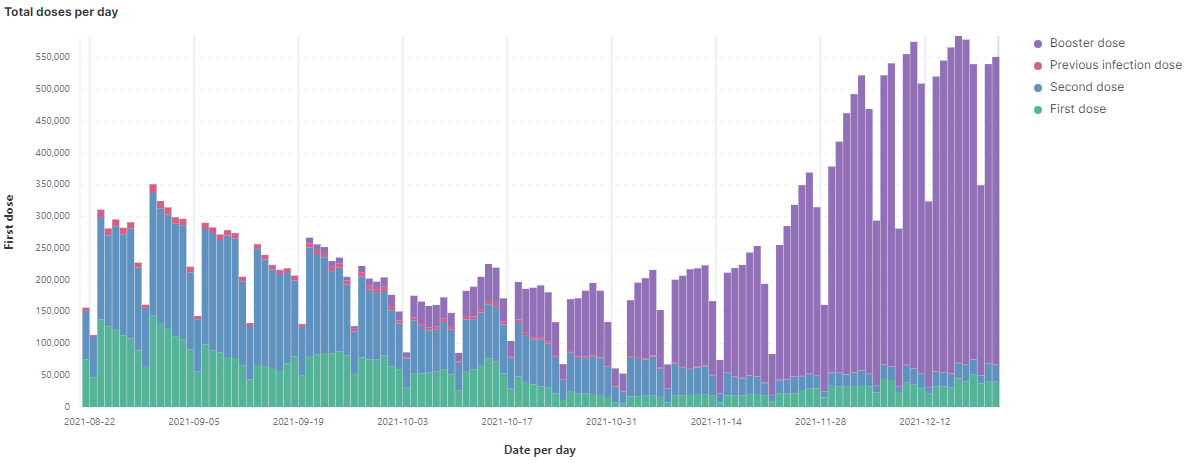
\includegraphics[width=\linewidth]{dashboards/dash1.png}
\end{figure}
\clearpage
\subsection{Total doses per region and provider in Italy}

\paragraph{}This representation is also derived from the second query and it shows for each vaccine provider the percentage of vaccinations for each region. We can focus on a specific region or a specific provider.\\
As we can see Astrazeneca in the last months has almost vanished, but if we extend the time horizon to the previous months the slice gets bigger
\begin{figure}[h]
	\centering
  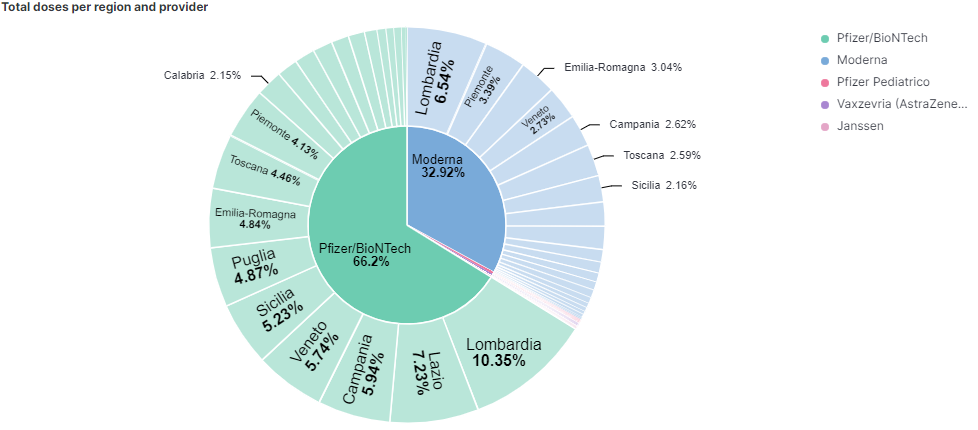
\includegraphics[width=\linewidth]{dashboards/dash2.png}
\end{figure}

\subsection{Total doses per age range and provider in Italy}

\paragraph{}This representation is derived from a generalization of the third query, it shows the total doses divided per age range and breaked down by vaccine type.
We can modify the time horizon as we please and focus on just a limited types of vaccinations or age ranges.\\
We can make the same conclusion about the Astrazeneca vaccine.
\begin{figure}[h]
	\centering
  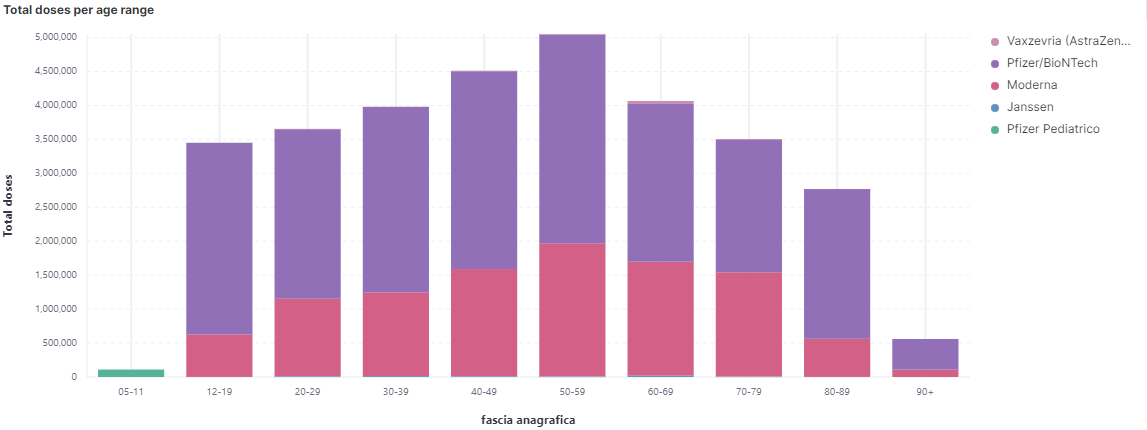
\includegraphics[width=\linewidth]{dashboards/dash3.png}
\end{figure}

\subsection{Gender comparison on total vaccinations in Italy}

\paragraph{}This representation shows the total vaccinations breaked down by vaccine type in percentage, between male and female. \\
We can focus on just one type of vaccine or gender.
\begin{figure}[h]
	\centering
  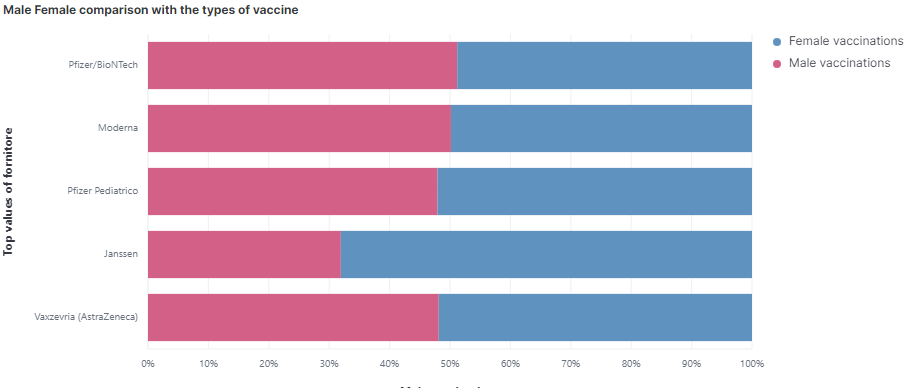
\includegraphics[width=\linewidth]{dashboards/dash4.png}
\end{figure}

\subsection{Trend of vaccines compared with deaths and infections in Italy}

\paragraph{}In this representation we mixed two different indexes ( vaccinations and global infections/deaths) in order to get a comparison of this data in Italy in the same graph.
\\
We can navigate the graph exploiting the informations of just one index for example hiding the information about the vaccinations to get a clearer graph about infections and deaths.
\begin{figure}[h]
	\centering
  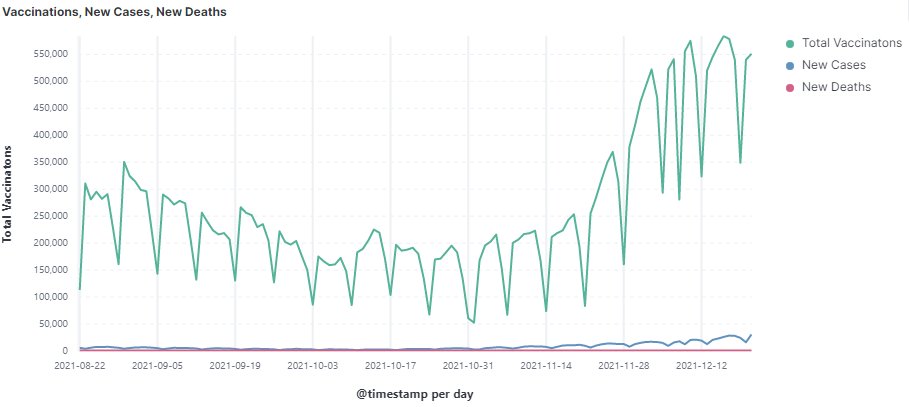
\includegraphics[width=\linewidth]{dashboards/dash5.png}
\end{figure}
\clearpage
\subsection{Trend of new cases in the world}

\paragraph{}In this representation we exploits the global index to get a trend of the continents new cases per million and we compare it with the new cases in Italy (red line).
\begin{figure}[h]
	\centering
  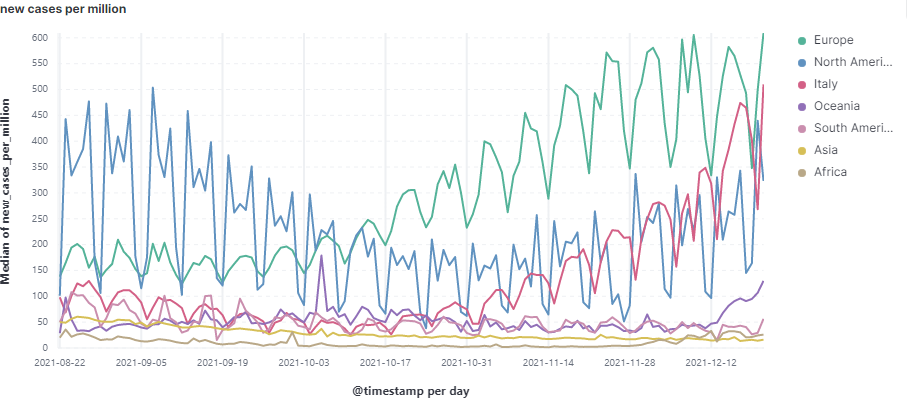
\includegraphics[width=\linewidth]{dashboards/dash6.png}
\end{figure}

\subsection{Trend of new cases in the italian regions}
\paragraph{}In this representation we exploits the regional infection index to get a trend of the italian regional new cases. \\ We can navigate the graph and select each region, or set of regions, one by one to get a clearer view of the trend.
\begin{figure}[h]
	\centering
  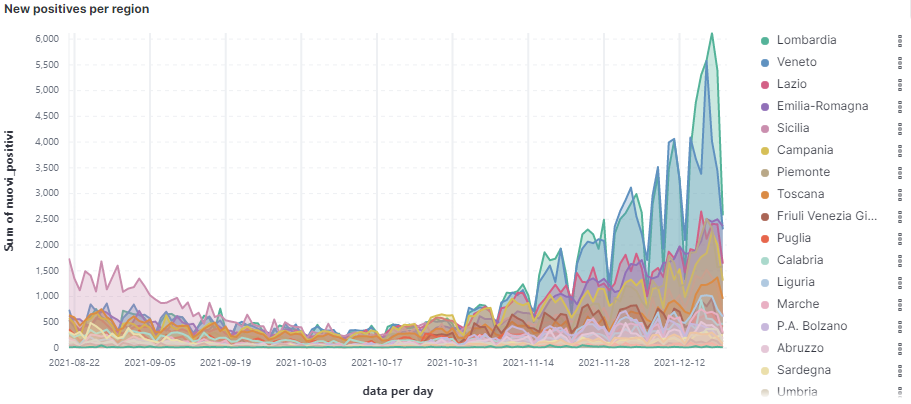
\includegraphics[width=\linewidth]{dashboards/dash7.png}
\end{figure}

\subsection{Trend of intensive care occupation and hospitalization in Italy}
\paragraph{}In this representation we exploits the regional infection index to get a trend of the hospitalization compared with the intensive care occupations. \\It is paramount important to keep checked this information in order to avoid health crisis.
\begin{figure}[h]
	\centering
  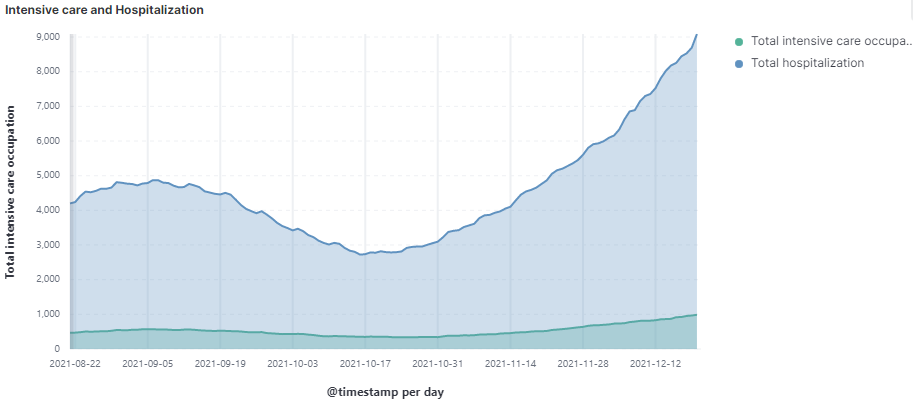
\includegraphics[width=\linewidth]{dashboards/dash8.png}
\end{figure}

\subsection{Mortality in the italian regions}
\paragraph{}In this representation we can compare the percentage mortality region by region.
It is interesting trying to understand the meaning behind this graph.
\begin{figure}[h]
	\centering
  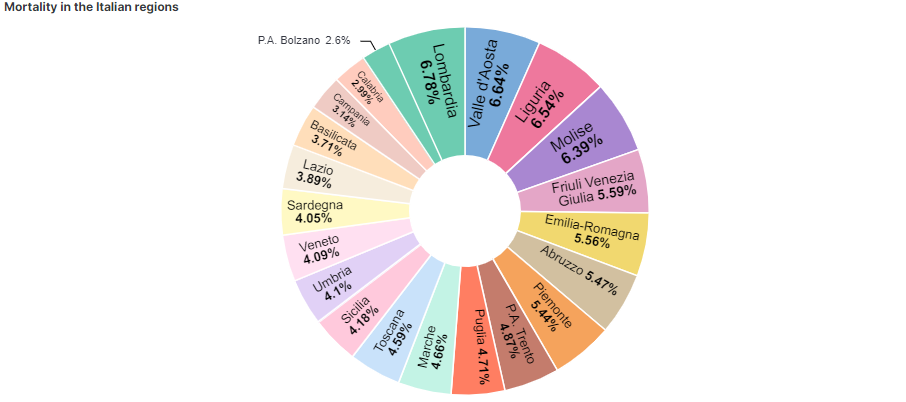
\includegraphics[width=\linewidth]{dashboards/dash9.png}
\end{figure}

\subsection{Variants percentage spread of variants in a given week}
\paragraph{}In this last representation we exploit the variants index in order to visualize the query number 8, that is, the spread on a pie chart of the variants in Italy the 32th week of the 2021.
\begin{figure}[h]
	\centering
  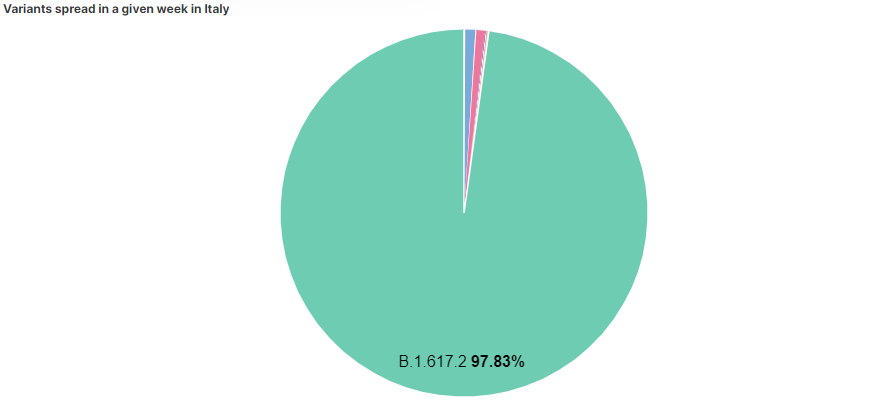
\includegraphics[width=\linewidth]{dashboards/dash10.png}
\end{figure}
\newpage

\section{References \& Sources}
  \begin{thebibliography}{9}
    \bibitem{} Course Slides
    \bibitem{} https://github.com/italia/covid19-opendata-vaccini/
    \bibitem{} https://www.ecdc.europa.eu/en/publications-data/data-virus-variants-covid-19-eueea
    \bibitem{} https://github.com/pcm-dpc/COVID-19
    \bibitem{} https://github.com/owid/covid-19-data
    \bibitem{} https://www.elastic.co/guide/en/elasticsearch/reference/current/index.html
  \end{thebibliography}
\end{document}
